\documentclass[12pt]{article}

\usepackage[utf8]{inputenc}
\usepackage[T1]{fontenc}
\usepackage[catalan]{babel}
\usepackage{lmodern}
\usepackage{geometry}
\usepackage{hyperref}
\usepackage{listings}
\usepackage{textcomp}
\usepackage[dvipsnames]{xcolor}
\usepackage[bf,sf,pagestyles]{titlesec}
\usepackage{titling}
\usepackage[font={footnotesize, sf}, labelfont=bf]{caption} 
\usepackage{siunitx}
\usepackage{graphicx}
\usepackage{booktabs}
\usepackage{amsmath,amssymb}
\usepackage[catalan,sort]{cleveref}
\usepackage{enumitem}

\lstdefinestyle{customc}{
  belowcaptionskip=1\baselineskip,
  breaklines=true,
	breakatwhitespace = true,
	postbreak = \textrightarrow\,,
  xleftmargin=\parindent,
	frame = l,
  language=C,
  showstringspaces=false,
  basicstyle=\small\ttfamily,
  keywordstyle=\bfseries\color{green!40!black},
  commentstyle=\sffamily\itshape\color{purple!40!black},
  identifierstyle=\color{blue},
  stringstyle=\color{orange},
	numbers = left, 
	numberstyle = \tiny\ttfamily,
}
\lstset{texcl=true,style=customc}
\renewcommand{\lstlistingname}{Programa}

\geometry{
	a4paper,
	right = 2.5cm,
	left = 2.5cm,
	bottom = 3cm,
	top = 3cm
}

\hypersetup{
	colorlinks,
	linkcolor = {red!50!blue},
	linktoc = page
}

\crefname{figure}{figura}{figures}
\crefname{table}{taula}{taules}
\numberwithin{table}{section}
\numberwithin{figure}{section}
\numberwithin{equation}{section}

\graphicspath{{./figs/}}

% Unitats
\sisetup{
	inter-unit-product = \ensuremath{ \, },
	allow-number-unit-breaks = true,
	math-celsius = {}^{\circ}\kern-\scriptspace C,
	detect-family = true,
	detect-shape = true,
	list-final-separator = { i },
	list-pair-separator = { i },
	list-units = single,
	separate-uncertainty = true
}

\DeclareMathAlphabet{\mathsfit}{T1}{\sfdefault}{\mddefault}{\sldefault}

\newcommand{\Z}{\mathbb{Z}}
\newcommand{\N}{\mathbb{N}}
\newcommand{\R}{\mathbb{R}}
\newcommand{\Ry}{\mathit{Ry}}
\newcommand{\data}[3]{\SI{#1 \pm #2}{#3}}
\newcommand{\unc}[2]{\ensuremath{{}\pm \SI{#1}{#2}}}
\DeclareMathOperator{\gr}{gr}
\newcommand{\abs}[1]{\left\lvert #1 \right\rvert}
\newcommand{\inn}[2]{\left\langle #1 , #2 \right\rangle}
\newcommand{\parbreak}{
	\begin{center}
		--- $\ast$ ---
	\end{center} 
}
\makeatletter
\newcommand*{\defeq}{\mathrel{\rlap{%
			\raisebox{0.3ex}{$\m@th\cdot$}}%
		\raisebox{-0.3ex}{$\m@th\cdot$}}%
	=
}
\makeatother

\newpagestyle{pagina}{
	\headrule
	\sethead*{\sffamily \bfseries Entrega 1}{}{\theauthor}
	\footrule
	\setfoot*{}{}{\sffamily \thepage}
}
\renewpagestyle{plain}{
	\footrule
	\setfoot*{}{}{\sffamily \thepage}
}
\pagestyle{pagina}

\title{\sffamily {\bfseries Entrega 1:} La temperatura d'un habitatge amb calefacció regulada per temporitzador}
\author{\sffamily Arnau Mas}
\date{\sffamily 27 de novembre de 2018}

\begin{document}
\maketitle
\section{Introducció}
Partim de la llei de Newton del refredament, \( \dot{T} = -k(T - T_e) \) on \( T_e \) és la temperatura ambient i \( k \) un coeficient relacionat amb la conductivitat del sistema ---com més petita és \( k \) més ben aïllat es troba el sistema---. Podem pensar que la temperatura ambient depèn del temps, així com introduir un terme de font, \( q \), potencialment també dependent del temps, que representa un flux de calor que rep el sistema. Així la nostra equació fonamental serà
\begin{equation} \label{eq:refredament}
	\dot{T} = q(t) - k(T - T_e(t)).
\end{equation}

Al llarg de tot l'informe suposarem que la temperatura ambient pren la forma
\begin{equation*}
	T_e(t) = \frac{1}{2}(T_\text{max} + T_\text{min}) + \frac{1}{2}(T_\text{max} - T_\text{min})\sin{\omega t},
\end{equation*}
és a dir, que varia entre \( T_\text{max} \) i \( T_\text{min} \) amb un període de \( \frac{2\pi}{\omega} \). Podem posar \( \bar{T} = \frac{1}{2}(T_\text{max} + T_\text{min}) \) i \( \Delta T = (T_\text{max} - T_\text{min}) \) i per tant \( T_e(t) = \bar{T} + \frac{1}{2}\Delta T \sin{\omega t} \). Així, si \( \omega = \frac{2\pi}{24} \), \( \bar{T} \) és la temperatura ambient mitjana i \( \Delta T \) la variació de temperatura total en un dia.

El nostre problema, doncs, és trobar un model per a la calefacció, és a dir, una forma per a \( q(t) \) que sigui òptima segons algun criteri.  

\section{Models senzills}
\subsection{Calefacció constant}
El model més senzill és considerar \( q_1(t) \) constant en el temps. L'\cref{eq:refredament} esdevé
\begin{equation*} 
	\dot{T} - kT = q_1 + \bar{T} + \frac{k\Delta T}{2}\sin{\omega t}.  
\end{equation*}
Aquesta equació es pot resoldre analíticament i resulta 
\begin{equation} \label{eq:solucio 1}
	T_1(t) = T_0e^{-kt} + \left(1 - e^{-kt}\right) \left(\frac{q_1}{k} + \bar{T}\right) + \frac{k \Delta T}{2(k^2 + \omega^2)}\left(k \sin{\omega t} - \omega \cos{\omega t} + \omega e^{-kt}\right),
\end{equation}
amb \( T_0 \) la temperatura inicial.

\begin{figure}[htb]
	\small \sffamily \centering
	% GNUPLOT: LaTeX picture with Postscript
\begingroup
\small
  \makeatletter
  \providecommand\color[2][]{%
    \GenericError{(gnuplot) \space\space\space\@spaces}{%
      Package color not loaded in conjunction with
      terminal option `colourtext'%
    }{See the gnuplot documentation for explanation.%
    }{Either use 'blacktext' in gnuplot or load the package
      color.sty in LaTeX.}%
    \renewcommand\color[2][]{}%
  }%
  \providecommand\includegraphics[2][]{%
    \GenericError{(gnuplot) \space\space\space\@spaces}{%
      Package graphicx or graphics not loaded%
    }{See the gnuplot documentation for explanation.%
    }{The gnuplot epslatex terminal needs graphicx.sty or graphics.sty.}%
    \renewcommand\includegraphics[2][]{}%
  }%
  \providecommand\rotatebox[2]{#2}%
  \@ifundefined{ifGPcolor}{%
    \newif\ifGPcolor
    \GPcolortrue
  }{}%
  \@ifundefined{ifGPblacktext}{%
    \newif\ifGPblacktext
    \GPblacktextfalse
  }{}%
  % define a \g@addto@macro without @ in the name:
  \let\gplgaddtomacro\g@addto@macro
  % define empty templates for all commands taking text:
  \gdef\gplbacktext{}%
  \gdef\gplfronttext{}%
  \makeatother
  \ifGPblacktext
    % no textcolor at all
    \def\colorrgb#1{}%
    \def\colorgray#1{}%
  \else
    % gray or color?
    \ifGPcolor
      \def\colorrgb#1{\color[rgb]{#1}}%
      \def\colorgray#1{\color[gray]{#1}}%
      \expandafter\def\csname LTw\endcsname{\color{white}}%
      \expandafter\def\csname LTb\endcsname{\color{black}}%
      \expandafter\def\csname LTa\endcsname{\color{black}}%
      \expandafter\def\csname LT0\endcsname{\color[rgb]{1,0,0}}%
      \expandafter\def\csname LT1\endcsname{\color[rgb]{0,1,0}}%
      \expandafter\def\csname LT2\endcsname{\color[rgb]{0,0,1}}%
      \expandafter\def\csname LT3\endcsname{\color[rgb]{1,0,1}}%
      \expandafter\def\csname LT4\endcsname{\color[rgb]{0,1,1}}%
      \expandafter\def\csname LT5\endcsname{\color[rgb]{1,1,0}}%
      \expandafter\def\csname LT6\endcsname{\color[rgb]{0,0,0}}%
      \expandafter\def\csname LT7\endcsname{\color[rgb]{1,0.3,0}}%
      \expandafter\def\csname LT8\endcsname{\color[rgb]{0.5,0.5,0.5}}%
    \else
      % gray
      \def\colorrgb#1{\color{black}}%
      \def\colorgray#1{\color[gray]{#1}}%
      \expandafter\def\csname LTw\endcsname{\color{white}}%
      \expandafter\def\csname LTb\endcsname{\color{black}}%
      \expandafter\def\csname LTa\endcsname{\color{black}}%
      \expandafter\def\csname LT0\endcsname{\color{black}}%
      \expandafter\def\csname LT1\endcsname{\color{black}}%
      \expandafter\def\csname LT2\endcsname{\color{black}}%
      \expandafter\def\csname LT3\endcsname{\color{black}}%
      \expandafter\def\csname LT4\endcsname{\color{black}}%
      \expandafter\def\csname LT5\endcsname{\color{black}}%
      \expandafter\def\csname LT6\endcsname{\color{black}}%
      \expandafter\def\csname LT7\endcsname{\color{black}}%
      \expandafter\def\csname LT8\endcsname{\color{black}}%
    \fi
  \fi
    \setlength{\unitlength}{0.0500bp}%
    \ifx\gptboxheight\undefined%
      \newlength{\gptboxheight}%
      \newlength{\gptboxwidth}%
      \newsavebox{\gptboxtext}%
    \fi%
    \setlength{\fboxrule}{0.5pt}%
    \setlength{\fboxsep}{1pt}%
\begin{picture}(5660.00,4520.00)%
    \gplgaddtomacro\gplbacktext{%
      \csname LTb\endcsname%%
      \put(1032,499){\makebox(0,0)[r]{\strut{}\num{10}}}%
      \csname LTb\endcsname%%
      \put(1032,1474){\makebox(0,0)[r]{\strut{}\num{15}}}%
      \csname LTb\endcsname%%
      \put(1032,2450){\makebox(0,0)[r]{\strut{}\num{20}}}%
      \csname LTb\endcsname%%
      \put(1032,3425){\makebox(0,0)[r]{\strut{}\num{25}}}%
      \csname LTb\endcsname%%
      \put(1032,4400){\makebox(0,0)[r]{\strut{}\num{30}}}%
      \csname LTb\endcsname%%
      \put(1132,321){\makebox(0,0){\strut{}\num{0}}}%
      \csname LTb\endcsname%%
      \put(2026,321){\makebox(0,0){\strut{}\num{2}}}%
      \csname LTb\endcsname%%
      \put(2920,321){\makebox(0,0){\strut{}\num{4}}}%
      \csname LTb\endcsname%%
      \put(3814,321){\makebox(0,0){\strut{}\num{6}}}%
      \csname LTb\endcsname%%
      \put(4708,321){\makebox(0,0){\strut{}\num{8}}}%
      \csname LTb\endcsname%%
      \put(5602,321){\makebox(0,0){\strut{}\num{10}}}%
    }%
    \gplgaddtomacro\gplfronttext{%
      \csname LTb\endcsname%%
      \put(544,2449){\rotatebox{-270}{\makebox(0,0){\strut{}$\mathsfit T$ (\si{\celsius})}}}%
      \csname LTb\endcsname%%
      \put(3367,83){\makebox(0,0){\strut{}$\mathsfit t$ (\si{dies})}}%
    }%
    \gplbacktext
    \put(0,0){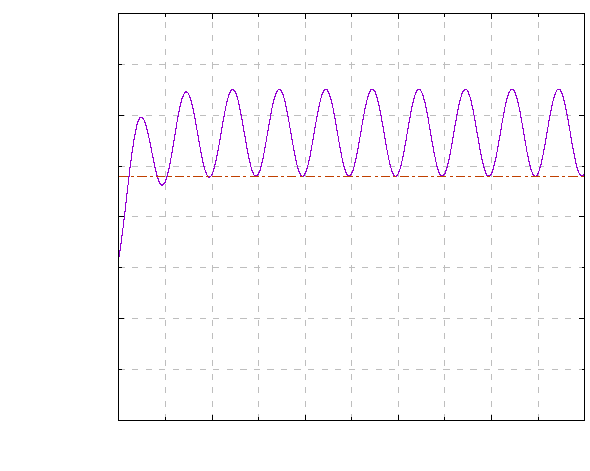
\includegraphics{model-1}}%
    \gplfronttext
  \end{picture}%
\endgroup

	\caption{Evolució de la temperatura de la casa amb un calefactor constantment encès de manera que la temperatura no baixi dels \SI{22}{\celsius}}
	\label{fig:sol 1}
\end{figure}

Per a \( t \) prou gran, tots els termes que tinguin una exponencial negativa es fan petits. Aquest límit s'anomena règim estacionari o permanent, i en aquest cas és
\begin{equation} \label{eq:estacionari 1}
	\begin{aligned}
		T_1^\text{est} (t) & = \frac{q_1}{k} + \bar{T} + \frac{k\Delta T}{2(k^2 + \omega^2)}\left(k \sin{\omega t} - \omega \cos{\omega t}\right) \\
										 	 & = \frac{q_1}{k} + \bar{T} + \frac{k\Delta T}{2\sqrt{k^2 + \omega^2}}\left(k \sin{\left(\omega t + \theta\right)}\right)
	\end{aligned}
\end{equation}
on \( \theta \) satisfà que \( \tan{\theta} = \frac{\omega}{k} \). 

Un requeriment raonable és que la temperatura sempre estigui per sobre d'una temperatura llindar \( T_l \). Podem imposar això només sobre el règim estacionari, ja que les fluctuacions de l'estat transitori, per a valors de \( k \) raonables, no duren més de 12 hores. Així hem de tenir
\begin{equation*}
	\frac{q_1}{k} + \bar{T} - \frac{k\Delta T}{2\sqrt{k^2 + \omega^2}} \geq T_l
\end{equation*}
i per tant el mínim valor que satisfà això és 
\begin{equation*}
	q_1 = k\left(T_l - \bar{T}\right) + \frac{k^2 \Delta T}{2 \sqrt{k^2 + \omega^2}}. 
\end{equation*}

A la \cref{fig:sol 1} es mostra la temperatura amb aquest model de calefacció. La temperatura inicial és de \SI{18}{\celsius} i \( k = \SI{0.1}{\celsius.s^{-1}} \). La temperatura ambient osci\l.la entre els \SI{8}{\celsius} i \SI{20}{\celsius}, i per tant \( q_1 \approx \SI{1.014}{\celsius.s^{-1}} \). 

\subsection{Model sinusoïdal}
\begin{figure}[htb]
	\small \sffamily \centering
	% GNUPLOT: LaTeX picture with Postscript
\begingroup
\small
  \makeatletter
  \providecommand\color[2][]{%
    \GenericError{(gnuplot) \space\space\space\@spaces}{%
      Package color not loaded in conjunction with
      terminal option `colourtext'%
    }{See the gnuplot documentation for explanation.%
    }{Either use 'blacktext' in gnuplot or load the package
      color.sty in LaTeX.}%
    \renewcommand\color[2][]{}%
  }%
  \providecommand\includegraphics[2][]{%
    \GenericError{(gnuplot) \space\space\space\@spaces}{%
      Package graphicx or graphics not loaded%
    }{See the gnuplot documentation for explanation.%
    }{The gnuplot epslatex terminal needs graphicx.sty or graphics.sty.}%
    \renewcommand\includegraphics[2][]{}%
  }%
  \providecommand\rotatebox[2]{#2}%
  \@ifundefined{ifGPcolor}{%
    \newif\ifGPcolor
    \GPcolortrue
  }{}%
  \@ifundefined{ifGPblacktext}{%
    \newif\ifGPblacktext
    \GPblacktextfalse
  }{}%
  % define a \g@addto@macro without @ in the name:
  \let\gplgaddtomacro\g@addto@macro
  % define empty templates for all commands taking text:
  \gdef\gplbacktext{}%
  \gdef\gplfronttext{}%
  \makeatother
  \ifGPblacktext
    % no textcolor at all
    \def\colorrgb#1{}%
    \def\colorgray#1{}%
  \else
    % gray or color?
    \ifGPcolor
      \def\colorrgb#1{\color[rgb]{#1}}%
      \def\colorgray#1{\color[gray]{#1}}%
      \expandafter\def\csname LTw\endcsname{\color{white}}%
      \expandafter\def\csname LTb\endcsname{\color{black}}%
      \expandafter\def\csname LTa\endcsname{\color{black}}%
      \expandafter\def\csname LT0\endcsname{\color[rgb]{1,0,0}}%
      \expandafter\def\csname LT1\endcsname{\color[rgb]{0,1,0}}%
      \expandafter\def\csname LT2\endcsname{\color[rgb]{0,0,1}}%
      \expandafter\def\csname LT3\endcsname{\color[rgb]{1,0,1}}%
      \expandafter\def\csname LT4\endcsname{\color[rgb]{0,1,1}}%
      \expandafter\def\csname LT5\endcsname{\color[rgb]{1,1,0}}%
      \expandafter\def\csname LT6\endcsname{\color[rgb]{0,0,0}}%
      \expandafter\def\csname LT7\endcsname{\color[rgb]{1,0.3,0}}%
      \expandafter\def\csname LT8\endcsname{\color[rgb]{0.5,0.5,0.5}}%
    \else
      % gray
      \def\colorrgb#1{\color{black}}%
      \def\colorgray#1{\color[gray]{#1}}%
      \expandafter\def\csname LTw\endcsname{\color{white}}%
      \expandafter\def\csname LTb\endcsname{\color{black}}%
      \expandafter\def\csname LTa\endcsname{\color{black}}%
      \expandafter\def\csname LT0\endcsname{\color{black}}%
      \expandafter\def\csname LT1\endcsname{\color{black}}%
      \expandafter\def\csname LT2\endcsname{\color{black}}%
      \expandafter\def\csname LT3\endcsname{\color{black}}%
      \expandafter\def\csname LT4\endcsname{\color{black}}%
      \expandafter\def\csname LT5\endcsname{\color{black}}%
      \expandafter\def\csname LT6\endcsname{\color{black}}%
      \expandafter\def\csname LT7\endcsname{\color{black}}%
      \expandafter\def\csname LT8\endcsname{\color{black}}%
    \fi
  \fi
    \setlength{\unitlength}{0.0500bp}%
    \ifx\gptboxheight\undefined%
      \newlength{\gptboxheight}%
      \newlength{\gptboxwidth}%
      \newsavebox{\gptboxtext}%
    \fi%
    \setlength{\fboxrule}{0.5pt}%
    \setlength{\fboxsep}{1pt}%
\begin{picture}(5660.00,4520.00)%
    \gplgaddtomacro\gplbacktext{%
      \csname LTb\endcsname%%
      \put(1032,499){\makebox(0,0)[r]{\strut{}\num{10}}}%
      \csname LTb\endcsname%%
      \put(1032,1474){\makebox(0,0)[r]{\strut{}\num{15}}}%
      \csname LTb\endcsname%%
      \put(1032,2450){\makebox(0,0)[r]{\strut{}\num{20}}}%
      \csname LTb\endcsname%%
      \put(1032,3425){\makebox(0,0)[r]{\strut{}\num{25}}}%
      \csname LTb\endcsname%%
      \put(1032,4400){\makebox(0,0)[r]{\strut{}\num{30}}}%
      \csname LTb\endcsname%%
      \put(1132,321){\makebox(0,0){\strut{}\num{0}}}%
      \csname LTb\endcsname%%
      \put(2026,321){\makebox(0,0){\strut{}\num{2}}}%
      \csname LTb\endcsname%%
      \put(2920,321){\makebox(0,0){\strut{}\num{4}}}%
      \csname LTb\endcsname%%
      \put(3814,321){\makebox(0,0){\strut{}\num{6}}}%
      \csname LTb\endcsname%%
      \put(4708,321){\makebox(0,0){\strut{}\num{8}}}%
      \csname LTb\endcsname%%
      \put(5602,321){\makebox(0,0){\strut{}\num{10}}}%
    }%
    \gplgaddtomacro\gplfronttext{%
      \csname LTb\endcsname%%
      \put(544,2449){\rotatebox{-270}{\makebox(0,0){\strut{}$\mathsfit T$ (\si{\celsius})}}}%
      \csname LTb\endcsname%%
      \put(3367,83){\makebox(0,0){\strut{}$\mathsfit t$ (\si{dies})}}%
    }%
    \gplbacktext
    \put(0,0){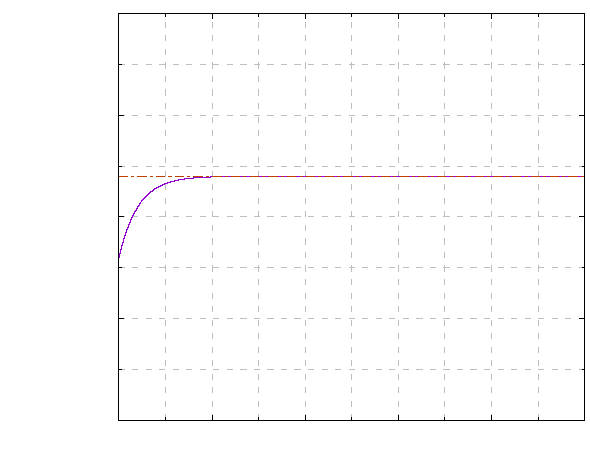
\includegraphics{model-2}}%
    \gplfronttext
  \end{picture}%
\endgroup

	\caption{Evolució de la temperatura de la casa amb un calefactor encès amb un patró sinusoïdal per mantenir la temperatura de la casa a \SI{22}{\celsius} de manera constant}
	\label{fig:sol 2}
\end{figure}

També podem requerir que el nostre calefactor anu\l.li les fluctuacions de la temperatura ambient tot mantenint la casa a una temperatura desitjada \( T_l \). Per a aconseguir això podem posar \( q_2(t) = kT_l - kT_e(t) \), de manera que l'\cref{eq:refredament} ara esdevé
\begin{equation*} 
	\dot{T} = -k(T - T_l).
\end{equation*}
Aquesta solució té una solució molt senzilla,
\begin{equation} \label{eq:solucio 2}
	T_2(t) = T_0e^{-kt} + \left(1 - e^{-kt}\right)T_l
\end{equation}
Com abans, tenim que per a valors raonables de \( k \), el terme transitori es fa molt petit durant les primeres 12 hores, de manera que \( T_2(t) \approx T_l \) a partir de llavors. 

A la \cref{fig:sol 2} es representa el perfil de temperatura que dóna aquest temporitzador, amb els mateixos paràmetres que a la secció anterior. 

\subsection{Comparació}
\begin{figure}[tb]
	\small \sffamily \centering
	% GNUPLOT: LaTeX picture with Postscript
\begingroup
\small
  \makeatletter
  \providecommand\color[2][]{%
    \GenericError{(gnuplot) \space\space\space\@spaces}{%
      Package color not loaded in conjunction with
      terminal option `colourtext'%
    }{See the gnuplot documentation for explanation.%
    }{Either use 'blacktext' in gnuplot or load the package
      color.sty in LaTeX.}%
    \renewcommand\color[2][]{}%
  }%
  \providecommand\includegraphics[2][]{%
    \GenericError{(gnuplot) \space\space\space\@spaces}{%
      Package graphicx or graphics not loaded%
    }{See the gnuplot documentation for explanation.%
    }{The gnuplot epslatex terminal needs graphicx.sty or graphics.sty.}%
    \renewcommand\includegraphics[2][]{}%
  }%
  \providecommand\rotatebox[2]{#2}%
  \@ifundefined{ifGPcolor}{%
    \newif\ifGPcolor
    \GPcolortrue
  }{}%
  \@ifundefined{ifGPblacktext}{%
    \newif\ifGPblacktext
    \GPblacktextfalse
  }{}%
  % define a \g@addto@macro without @ in the name:
  \let\gplgaddtomacro\g@addto@macro
  % define empty templates for all commands taking text:
  \gdef\gplbacktext{}%
  \gdef\gplfronttext{}%
  \makeatother
  \ifGPblacktext
    % no textcolor at all
    \def\colorrgb#1{}%
    \def\colorgray#1{}%
  \else
    % gray or color?
    \ifGPcolor
      \def\colorrgb#1{\color[rgb]{#1}}%
      \def\colorgray#1{\color[gray]{#1}}%
      \expandafter\def\csname LTw\endcsname{\color{white}}%
      \expandafter\def\csname LTb\endcsname{\color{black}}%
      \expandafter\def\csname LTa\endcsname{\color{black}}%
      \expandafter\def\csname LT0\endcsname{\color[rgb]{1,0,0}}%
      \expandafter\def\csname LT1\endcsname{\color[rgb]{0,1,0}}%
      \expandafter\def\csname LT2\endcsname{\color[rgb]{0,0,1}}%
      \expandafter\def\csname LT3\endcsname{\color[rgb]{1,0,1}}%
      \expandafter\def\csname LT4\endcsname{\color[rgb]{0,1,1}}%
      \expandafter\def\csname LT5\endcsname{\color[rgb]{1,1,0}}%
      \expandafter\def\csname LT6\endcsname{\color[rgb]{0,0,0}}%
      \expandafter\def\csname LT7\endcsname{\color[rgb]{1,0.3,0}}%
      \expandafter\def\csname LT8\endcsname{\color[rgb]{0.5,0.5,0.5}}%
    \else
      % gray
      \def\colorrgb#1{\color{black}}%
      \def\colorgray#1{\color[gray]{#1}}%
      \expandafter\def\csname LTw\endcsname{\color{white}}%
      \expandafter\def\csname LTb\endcsname{\color{black}}%
      \expandafter\def\csname LTa\endcsname{\color{black}}%
      \expandafter\def\csname LT0\endcsname{\color{black}}%
      \expandafter\def\csname LT1\endcsname{\color{black}}%
      \expandafter\def\csname LT2\endcsname{\color{black}}%
      \expandafter\def\csname LT3\endcsname{\color{black}}%
      \expandafter\def\csname LT4\endcsname{\color{black}}%
      \expandafter\def\csname LT5\endcsname{\color{black}}%
      \expandafter\def\csname LT6\endcsname{\color{black}}%
      \expandafter\def\csname LT7\endcsname{\color{black}}%
      \expandafter\def\csname LT8\endcsname{\color{black}}%
    \fi
  \fi
    \setlength{\unitlength}{0.0500bp}%
    \ifx\gptboxheight\undefined%
      \newlength{\gptboxheight}%
      \newlength{\gptboxwidth}%
      \newsavebox{\gptboxtext}%
    \fi%
    \setlength{\fboxrule}{0.5pt}%
    \setlength{\fboxsep}{1pt}%
\begin{picture}(5660.00,4520.00)%
    \gplgaddtomacro\gplbacktext{%
      \csname LTb\endcsname%%
      \put(1032,499){\makebox(0,0)[r]{\strut{}\num{10}}}%
      \csname LTb\endcsname%%
      \put(1032,1474){\makebox(0,0)[r]{\strut{}\num{15}}}%
      \csname LTb\endcsname%%
      \put(1032,2450){\makebox(0,0)[r]{\strut{}\num{20}}}%
      \csname LTb\endcsname%%
      \put(1032,3425){\makebox(0,0)[r]{\strut{}\num{25}}}%
      \csname LTb\endcsname%%
      \put(1032,4400){\makebox(0,0)[r]{\strut{}\num{30}}}%
      \csname LTb\endcsname%%
      \put(1132,321){\makebox(0,0){\strut{}\num{0}}}%
      \csname LTb\endcsname%%
      \put(2026,321){\makebox(0,0){\strut{}\num{2}}}%
      \csname LTb\endcsname%%
      \put(2920,321){\makebox(0,0){\strut{}\num{4}}}%
      \csname LTb\endcsname%%
      \put(3814,321){\makebox(0,0){\strut{}\num{6}}}%
      \csname LTb\endcsname%%
      \put(4708,321){\makebox(0,0){\strut{}\num{8}}}%
      \csname LTb\endcsname%%
      \put(5602,321){\makebox(0,0){\strut{}\num{10}}}%
    }%
    \gplgaddtomacro\gplfronttext{%
      \csname LTb\endcsname%%
      \put(544,2449){\rotatebox{-270}{\makebox(0,0){\strut{}$\mathsfit T$ (\si{\celsius})}}}%
      \csname LTb\endcsname%%
      \put(3367,83){\makebox(0,0){\strut{}$\mathsfit t$ (\si{dies})}}%
    }%
    \gplbacktext
    \put(0,0){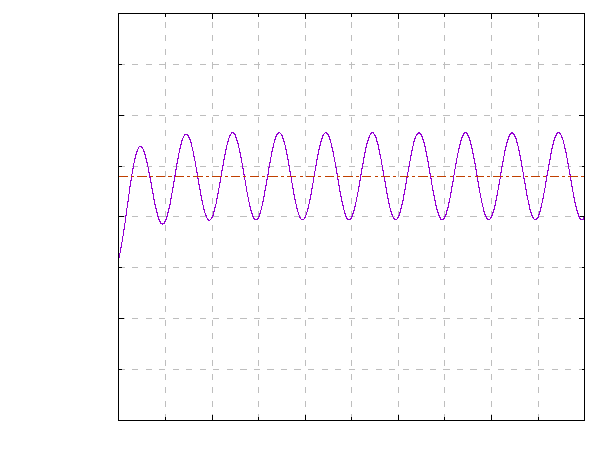
\includegraphics{model-3}}%
    \gplfronttext
  \end{picture}%
\endgroup

	\caption{Evolució de la temperatura de la casa amb un calefactor encès constantment per mantenir la temperatura de la casa osci\l.lant \SI{22}{\celsius} de manera constant}
	\label{fig:sol 3}
\end{figure}

Una bona manera de de comparar els diferents models és avaluar la integral
\begin{equation*}
	Q =	\int_0^{2\pi \omega} q(t) \, dt,
\end{equation*}
que és proporcional a la despesa energètica d'un dia, ja que, llevat de constants, \( q \) representa un flux de calor.   

Suposem que volem que la temperatura de la casa no superi una temperatura llindar \( T_l \). Aleshores, per a la calor constant \( q_1 \) tenim
\begin{equation} \label{eq:consum 1}
	Q_1 = \int_0^{2\pi \omega} q_1(t) \, dt = 2\pi\omega k(T_l - \bar{T}) + \frac{k^2 \Delta T}{\sqrt{k^2 + \omega^2}} \pi \omega.
\end{equation}

\begin{figure}[htb]
	\small \sffamily \centering
	% GNUPLOT: LaTeX picture with Postscript
\begingroup
\newcommand{\etiqueta}[1]{\setlength{\fboxsep}{0.75pt}\colorbox{white}{#1}}
  \makeatletter
  \providecommand\color[2][]{%
    \GenericError{(gnuplot) \space\space\space\@spaces}{%
      Package color not loaded in conjunction with
      terminal option `colourtext'%
    }{See the gnuplot documentation for explanation.%
    }{Either use 'blacktext' in gnuplot or load the package
      color.sty in LaTeX.}%
    \renewcommand\color[2][]{}%
  }%
  \providecommand\includegraphics[2][]{%
    \GenericError{(gnuplot) \space\space\space\@spaces}{%
      Package graphicx or graphics not loaded%
    }{See the gnuplot documentation for explanation.%
    }{The gnuplot epslatex terminal needs graphicx.sty or graphics.sty.}%
    \renewcommand\includegraphics[2][]{}%
  }%
  \providecommand\rotatebox[2]{#2}%
  \@ifundefined{ifGPcolor}{%
    \newif\ifGPcolor
    \GPcolortrue
  }{}%
  \@ifundefined{ifGPblacktext}{%
    \newif\ifGPblacktext
    \GPblacktextfalse
  }{}%
  % define a \g@addto@macro without @ in the name:
  \let\gplgaddtomacro\g@addto@macro
  % define empty templates for all commands taking text:
  \gdef\gplbacktext{}%
  \gdef\gplfronttext{}%
  \makeatother
  \ifGPblacktext
    % no textcolor at all
    \def\colorrgb#1{}%
    \def\colorgray#1{}%
  \else
    % gray or color?
    \ifGPcolor
      \def\colorrgb#1{\color[rgb]{#1}}%
      \def\colorgray#1{\color[gray]{#1}}%
      \expandafter\def\csname LTw\endcsname{\color{white}}%
      \expandafter\def\csname LTb\endcsname{\color{black}}%
      \expandafter\def\csname LTa\endcsname{\color{black}}%
      \expandafter\def\csname LT0\endcsname{\color[rgb]{1,0,0}}%
      \expandafter\def\csname LT1\endcsname{\color[rgb]{0,1,0}}%
      \expandafter\def\csname LT2\endcsname{\color[rgb]{0,0,1}}%
      \expandafter\def\csname LT3\endcsname{\color[rgb]{1,0,1}}%
      \expandafter\def\csname LT4\endcsname{\color[rgb]{0,1,1}}%
      \expandafter\def\csname LT5\endcsname{\color[rgb]{1,1,0}}%
      \expandafter\def\csname LT6\endcsname{\color[rgb]{0,0,0}}%
      \expandafter\def\csname LT7\endcsname{\color[rgb]{1,0.3,0}}%
      \expandafter\def\csname LT8\endcsname{\color[rgb]{0.5,0.5,0.5}}%
    \else
      % gray
      \def\colorrgb#1{\color{black}}%
      \def\colorgray#1{\color[gray]{#1}}%
      \expandafter\def\csname LTw\endcsname{\color{white}}%
      \expandafter\def\csname LTb\endcsname{\color{black}}%
      \expandafter\def\csname LTa\endcsname{\color{black}}%
      \expandafter\def\csname LT0\endcsname{\color{black}}%
      \expandafter\def\csname LT1\endcsname{\color{black}}%
      \expandafter\def\csname LT2\endcsname{\color{black}}%
      \expandafter\def\csname LT3\endcsname{\color{black}}%
      \expandafter\def\csname LT4\endcsname{\color{black}}%
      \expandafter\def\csname LT5\endcsname{\color{black}}%
      \expandafter\def\csname LT6\endcsname{\color{black}}%
      \expandafter\def\csname LT7\endcsname{\color{black}}%
      \expandafter\def\csname LT8\endcsname{\color{black}}%
    \fi
  \fi
    \setlength{\unitlength}{0.0500bp}%
    \ifx\gptboxheight\undefined%
      \newlength{\gptboxheight}%
      \newlength{\gptboxwidth}%
      \newsavebox{\gptboxtext}%
    \fi%
    \setlength{\fboxrule}{0.5pt}%
    \setlength{\fboxsep}{1pt}%
\begin{picture}(5660.00,4520.00)%
    \gplgaddtomacro\gplbacktext{%
      \csname LTb\endcsname%%
      \put(1032,499){\makebox(0,0)[r]{\strut{}\num{0}}}%
      \csname LTb\endcsname%%
      \put(1032,1474){\makebox(0,0)[r]{\strut{}\num{0.5}}}%
      \csname LTb\endcsname%%
      \put(1032,2450){\makebox(0,0)[r]{\strut{}\num{1}}}%
      \csname LTb\endcsname%%
      \put(1032,3425){\makebox(0,0)[r]{\strut{}\num{1.5}}}%
      \csname LTb\endcsname%%
      \put(1032,4400){\makebox(0,0)[r]{\strut{}\num{2}}}%
      \csname LTb\endcsname%%
      \put(1132,321){\makebox(0,0){\strut{}\num{0}}}%
      \csname LTb\endcsname%%
      \put(2063,321){\makebox(0,0){\strut{}\num{5}}}%
      \csname LTb\endcsname%%
      \put(2995,321){\makebox(0,0){\strut{}\num{10}}}%
      \csname LTb\endcsname%%
      \put(3926,321){\makebox(0,0){\strut{}\num{15}}}%
      \csname LTb\endcsname%%
      \put(4857,321){\makebox(0,0){\strut{}\num{20}}}%
    }%
    \gplgaddtomacro\gplfronttext{%
      \csname LTb\endcsname%%
      \put(477,2449){\rotatebox{-270}{\makebox(0,0){\strut{}$\mathsfit q$ (\si{\celsius.s^{-1}})}}}%
      \csname LTb\endcsname%%
      \put(3367,83){\makebox(0,0){\strut{}$\mathsfit t$ (\si{h})}}%
      \colorrgb{0.58,0.00,0.83}%%
      \put(1598,2508){\makebox(0,0){\strut{}\etiqueta{\normalsize $\mathsfit q_\text{1}$}}}%
      \colorrgb{0.13,0.55,0.13}%%
      \put(1598,2059){\makebox(0,0){\strut{}\etiqueta{\normalsize $\mathsfit q'_\text{1}$}}}%
      \colorrgb{0.75,0.25,0.00}%%
      \put(1598,1377){\rotatebox{-45}{\makebox(0,0){\strut{}\etiqueta{\normalsize $\mathsfit q_\text{2}$}}}}%
    }%
    \gplbacktext
    \put(0,0){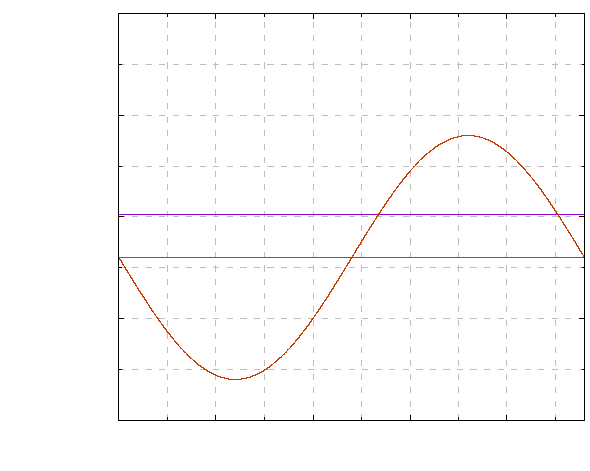
\includegraphics{calors}}%
    \gplfronttext
  \end{picture}%
\endgroup

	\caption{Perfils dels tres diferents models de calefacció}
	\label{fig:calors}
\end{figure}

Podem fer el mateix càlcul per al model sinusoïdal que manté la temperatura constant, \( q_2 \):
\begin{equation} \label{eq:consum 2}
	\begin{aligned}
		Q_2 & = \int_0^{2\pi \omega} q_2(t) \, dt = 2\pi\omega k(T_l - \bar{T}) - \frac{k \Delta T}{2} \int_0^{2\pi \omega} \sin{\omega t} \, dt \\
				& = 2\pi\omega k(T_l - \bar{T})
	\end{aligned}
\end{equation}
Veiem, doncs que \( Q_2 \leq Q_1 \), per tant el segon mètode és més eficaç, no només perquè consumeix menys, sino perquè manté una temperatura constant. 

Ara bé, podem ser més permissius i demanar no que la temperatura estigui per sobre d'un llindar, sino que oscil·li al voltant d'una temperatura determinada \( T_l \). Ja hem vist, \cref{eq:estacionari 1}, que el règim estacionari quan la calefacció és constant és una osci\l.lació al voltant de \( \frac{1}{k}q_1 + \bar{T} \). Per tant si demanem que aquesta temperatura sigui \( T_l \) obtenim
\begin{equation*}
	q_1' = k(T_1 - \bar{T}).
\end{equation*}
El consum diari ara és \( Q_1' = 2\pi\omega k(T_1 - \bar{T}) \), el mateix que amb el model de calefacció sinusoïdal. Veiem, doncs, que amb el mateix cost energètic tenim dues opcions: o bé mantenim una temperatura de la casa constant però, per contra, tenim un temporitzador complex, o bé permetem osci\l.lacions de la temperatura durant el dia a canvi de mantenir la calefacció a un valor constant. Aquest perfil es mostra a la \cref{fig:sol 3}.

A la \cref{fig:calors} es mostren els diferents perfils d'encès per als models proposats.

Val a dir que aquest model és extremadament simplificat, per tant les opcions que presentem no necessàriament s'ajusten al comportament real d'un sistema de calefacció d'un habitatge. 

\section{Termòstat}
\begin{figure}[tb]
	\small \sffamily \centering
	% GNUPLOT: LaTeX picture with Postscript
\begingroup
\small
  \makeatletter
  \providecommand\color[2][]{%
    \GenericError{(gnuplot) \space\space\space\@spaces}{%
      Package color not loaded in conjunction with
      terminal option `colourtext'%
    }{See the gnuplot documentation for explanation.%
    }{Either use 'blacktext' in gnuplot or load the package
      color.sty in LaTeX.}%
    \renewcommand\color[2][]{}%
  }%
  \providecommand\includegraphics[2][]{%
    \GenericError{(gnuplot) \space\space\space\@spaces}{%
      Package graphicx or graphics not loaded%
    }{See the gnuplot documentation for explanation.%
    }{The gnuplot epslatex terminal needs graphicx.sty or graphics.sty.}%
    \renewcommand\includegraphics[2][]{}%
  }%
  \providecommand\rotatebox[2]{#2}%
  \@ifundefined{ifGPcolor}{%
    \newif\ifGPcolor
    \GPcolortrue
  }{}%
  \@ifundefined{ifGPblacktext}{%
    \newif\ifGPblacktext
    \GPblacktextfalse
  }{}%
  % define a \g@addto@macro without @ in the name:
  \let\gplgaddtomacro\g@addto@macro
  % define empty templates for all commands taking text:
  \gdef\gplbacktext{}%
  \gdef\gplfronttext{}%
  \makeatother
  \ifGPblacktext
    % no textcolor at all
    \def\colorrgb#1{}%
    \def\colorgray#1{}%
  \else
    % gray or color?
    \ifGPcolor
      \def\colorrgb#1{\color[rgb]{#1}}%
      \def\colorgray#1{\color[gray]{#1}}%
      \expandafter\def\csname LTw\endcsname{\color{white}}%
      \expandafter\def\csname LTb\endcsname{\color{black}}%
      \expandafter\def\csname LTa\endcsname{\color{black}}%
      \expandafter\def\csname LT0\endcsname{\color[rgb]{1,0,0}}%
      \expandafter\def\csname LT1\endcsname{\color[rgb]{0,1,0}}%
      \expandafter\def\csname LT2\endcsname{\color[rgb]{0,0,1}}%
      \expandafter\def\csname LT3\endcsname{\color[rgb]{1,0,1}}%
      \expandafter\def\csname LT4\endcsname{\color[rgb]{0,1,1}}%
      \expandafter\def\csname LT5\endcsname{\color[rgb]{1,1,0}}%
      \expandafter\def\csname LT6\endcsname{\color[rgb]{0,0,0}}%
      \expandafter\def\csname LT7\endcsname{\color[rgb]{1,0.3,0}}%
      \expandafter\def\csname LT8\endcsname{\color[rgb]{0.5,0.5,0.5}}%
    \else
      % gray
      \def\colorrgb#1{\color{black}}%
      \def\colorgray#1{\color[gray]{#1}}%
      \expandafter\def\csname LTw\endcsname{\color{white}}%
      \expandafter\def\csname LTb\endcsname{\color{black}}%
      \expandafter\def\csname LTa\endcsname{\color{black}}%
      \expandafter\def\csname LT0\endcsname{\color{black}}%
      \expandafter\def\csname LT1\endcsname{\color{black}}%
      \expandafter\def\csname LT2\endcsname{\color{black}}%
      \expandafter\def\csname LT3\endcsname{\color{black}}%
      \expandafter\def\csname LT4\endcsname{\color{black}}%
      \expandafter\def\csname LT5\endcsname{\color{black}}%
      \expandafter\def\csname LT6\endcsname{\color{black}}%
      \expandafter\def\csname LT7\endcsname{\color{black}}%
      \expandafter\def\csname LT8\endcsname{\color{black}}%
    \fi
  \fi
    \setlength{\unitlength}{0.0500bp}%
    \ifx\gptboxheight\undefined%
      \newlength{\gptboxheight}%
      \newlength{\gptboxwidth}%
      \newsavebox{\gptboxtext}%
    \fi%
    \setlength{\fboxrule}{0.5pt}%
    \setlength{\fboxsep}{1pt}%
\begin{picture}(5660.00,4520.00)%
    \gplgaddtomacro\gplbacktext{%
      \csname LTb\endcsname%%
      \put(1032,499){\makebox(0,0)[r]{\strut{}\num{10}}}%
      \csname LTb\endcsname%%
      \put(1032,1474){\makebox(0,0)[r]{\strut{}\num{15}}}%
      \csname LTb\endcsname%%
      \put(1032,2450){\makebox(0,0)[r]{\strut{}\num{20}}}%
      \csname LTb\endcsname%%
      \put(1032,3425){\makebox(0,0)[r]{\strut{}\num{25}}}%
      \csname LTb\endcsname%%
      \put(1032,4400){\makebox(0,0)[r]{\strut{}\num{30}}}%
      \csname LTb\endcsname%%
      \put(1132,321){\makebox(0,0){\strut{}\num{0}}}%
      \csname LTb\endcsname%%
      \put(2026,321){\makebox(0,0){\strut{}\num{2}}}%
      \csname LTb\endcsname%%
      \put(2920,321){\makebox(0,0){\strut{}\num{4}}}%
      \csname LTb\endcsname%%
      \put(3814,321){\makebox(0,0){\strut{}\num{6}}}%
      \csname LTb\endcsname%%
      \put(4708,321){\makebox(0,0){\strut{}\num{8}}}%
      \csname LTb\endcsname%%
      \put(5602,321){\makebox(0,0){\strut{}\num{10}}}%
    }%
    \gplgaddtomacro\gplfronttext{%
      \csname LTb\endcsname%%
      \put(544,2449){\rotatebox{-270}{\makebox(0,0){\strut{}$\mathsfit T$ (\si{\celsius})}}}%
      \csname LTb\endcsname%%
      \put(3367,83){\makebox(0,0){\strut{}$\mathsfit t$ (\si{dies})}}%
    }%
    \gplbacktext
    \put(0,0){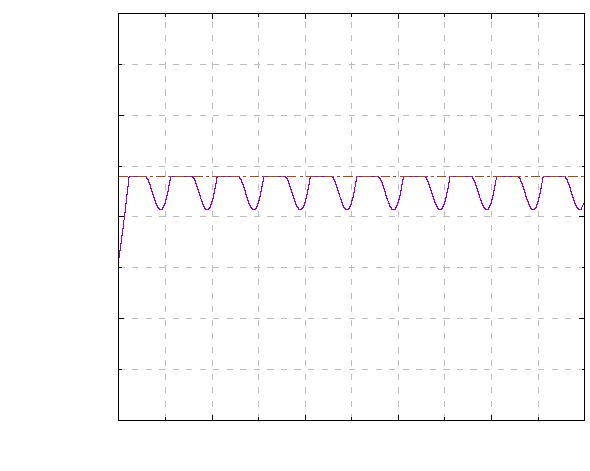
\includegraphics{model-4}}%
    \gplfronttext
  \end{picture}%
\endgroup

	\caption{Evolució de la temperatura incorporant una funció de Heaviside amb temperatura llindar \SI{22}{\celsius}}
	\label{fig:sol 4}
\end{figure}

Un model més realista consisteix en introduir un termòstat, és a dir, un sistema que encén el dispositiu calefactor només quan la temperatura baixa d'un cert valor llindar. Una manera de modelar això és amb la funció de Heaviside, que es defineix com \( H(x) = 1 \) per \( x \leq 0 \) i \( H(x) = 0 \) per \( x < 0 \). Aleshores, si fem \( q_3 = qH(T_l - T) \) estem modelant un termòstat que encendrà la calefacció quan \( T \leq T_l \). L'equació diferencial és
\begin{equation*}
	\dot{T} = -k(T - T_e(t)) + qH(T_l - T).
\end{equation*}
Sagemath no pot resoldre explícitament aquesta equació, però si que ho pot fer numèricament. A la \cref{fig:sol 4} es mostra el resultat de la integració numèrica. 

Com veiem, la temperatura no excedeix els \SI{22}{\celsius}, que és la temperatura llindar. Les baixades de temperatura periòdiques es minimitzen variant el valor del factor \( q \), que en el cas de la figura és 1. Només amb \( q = 1.5 \) la temperatura ja és manté essencialment constant a la temperatura llindar. Observem també que aquesta opció presenta molta menys osci\l.lació que el model amb \( q \) constant, la temperatura només es mou entre \SI{22}{\celsius} i \SI{20}{\celsius}. El consum energètic és molt similar al de \( q_1 \), ja que \( q_3 \) és o bé 0 o bé 1 i \( q_1 \) és molt propera a 1, però presenta molta menys osci\l.lació.

Aquest model és més realista ja que es podria adaptar a una temperatura ambient diferent, per exemple, que variés de forma estocàstica durant el dia. Els tres models anteriors depenien fortament de com hem modelat la temperatura ambient.

\appendix
\section{Codis}
\begin{lstlisting}[language=python, caption=Codi per simular el model amb \( q_1 \), label={lst:codi 1}]
# Donem valor als paràmetres
T_max = 20
T_min = 8
w = pi/12
k = 0.1

# Definim l'equació diferencial i la resolem
var('T_0, q')
T_e(t) = 0.5*(T_max + T_min) + 0.5*(T_max - T_min)*sin(w*t)
x = function('T')(t)
eq1 = diff(x,t) == q - k*(x - T_e(t))
T_1(t) = desolve(eq1, x, ivar = t, ics = [0,T_0])
q1 = 22*k - k*(T_max + T_min)/2 + k**2*(T_max - T_min)/(2*sqrt(k**2 + w**2))

# Fem el gràfic de la solució
plot(T_1.subs(q = q1, T_0 = 18), xmin = 0, xmax = 240) + plot(22, xmin = 0, xmax = 240, color = 'green', linestyle = '--')
\end{lstlisting}

\begin{lstlisting}[language=python, caption=Codi per simular el model amb \( q_2 \), label={lst:codi 2}]
# Donem valor als paràmetres
T_max = 20
T_min = 8
w = pi/12
k = 0.1

# Definim l'equació diferencial i la resolem
var('T_0, q')
T_e(t) = 0.5*(T_max + T_min) + 0.5*(T_max - T_min)*sin(w*t)
q2(t) = k*22 - k*T_e(t)
x = function('T')(t)
eq2 = diff(x,t) == q2(t) - k*(x - T_e(t))
T_2(t) = desolve(eq2, x, ivar = t, ics = [0,T_0])

# Fem el gràfic de la solució
plot(T_2.subs(T_0 = 18), xmin = 0, xmax = 240) + plot(22, xmin = 0, xmax = 240, color = 'green', linestyle = '--')
\end{lstlisting}

\begin{lstlisting}[language=python, caption=Codi per simular el model amb \( q_1' \), label={lst:codi 3}]
# Donem valor als paràmetres
T_max = 20
T_min = 8
w = pi/12
k = 0.1

# Definim l'equació diferencial i la resolem
var('T_0, q')
T_e(t) = 0.5*(T_max + T_min) + 0.5*(T_max - T_min)*sin(w*t)
x = function('T')(t)
eq3 = diff(x,t) == q - k*(x - T_e(t))
T_3(t) = desolve(eq3, x, ivar = t, ics = [0,T_0])
q3 = 22*k - k*(T_max + T_min)/2

# Fem el gràfic de la solució
plot(T_3.subs(q = q3, T_0 = 18), xmin = 0, xmax = 240) + plot(22, xmin = 0, xmax = 240, color = 'green', linestyle = '--')
\end{lstlisting}

\begin{lstlisting}[language=python, caption=Codi per simular el model amb \( q_3 \), label={lst:codi 4}]
# Donem valor als paràmetres
T_max = 20
T_min = 8
w = pi/12
k = 0.1

# Definim l'equació diferencial i la resolem
T_e(t) = 0.5*(T_max + T_min) + 0.5*(T_max - T_min)*sin(w*t)
x = function('T')(t)
eq4 = diff(x,t) == unit_step(22 - x) - k*(x - T_e(t))
punts = desolve_rk4(eq4, x, ivar = t, ics = [0,18], end_points = 240, step = 0.01)

# Fem el gràfic de la solució
list_plot(punts)
\end{lstlisting}

\end{document}
